% Patch 0103: CMYK colours converted like a PDF viewer does (MuPDF's CMYK profile), not with 1 - c - k.
% Text colours (color specials), \colorbox, TikZ fills and strokes (pdf:code k / K), and xcolor's named CMYK colours.
% Compare with Tectonic's PDF drawn by mutool.
\documentclass{article}
\usepackage{tikz}
\pagestyle{empty}
\begin{document}
{\Huge\bfseries
\color{yellow} yellow \color{cyan} cyan \color{magenta} magenta \color{olive} olive\par
\color[cmyk]{0.2,0.7,0.1,0.3} plum \color[cmyk]{0,0,0,0.5} grey \color[cmyk]{1,1,1,1} rich\par}
\colorbox{yellow}{\Huge on yellow}\ \fcolorbox[cmyk]{1,0,0,0}{0,0.5,0.9,0}{\Huge framed}

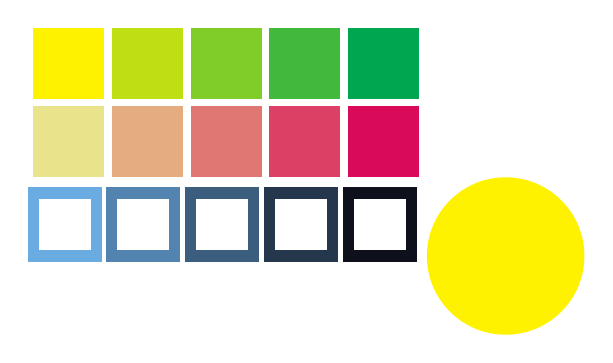
\begin{tikzpicture}
  \foreach \c [count=\i] in {0, 0.25, 0.5, 0.75, 1} {
    \definecolor{a}{cmyk}{\c,0,1,0}  \fill[a] (\i,0) rectangle +(0.9,0.9);
    \definecolor{b}{cmyk}{0,\c,0.4,0.1} \fill[b] (\i,-1) rectangle +(0.9,0.9);
    \definecolor{d}{cmyk}{0.6,0.2,0,\c} \draw[d, line width=4pt] (\i,-2) rectangle +(0.8,0.8);
  }
  \fill[yellow] (7,-2) circle (1);
\end{tikzpicture}
\end{document}
